\documentclass[11pt]{article}
\usepackage[T1]{fontenc}
\usepackage{lmodern}
\usepackage[margin=1in]{geometry}
\usepackage{amsmath,amssymb,amsthm,mathtools}
\usepackage{microtype,booktabs,array,enumitem}
\usepackage{tikz}
\usetikzlibrary{arrows.meta,calc,positioning}
\usepackage[hyphens]{url}
\usepackage[colorlinks=true,linkcolor=black,citecolor=black,urlcolor=black]{hyperref}
\usepackage{bookmark}
\bookmarksetup{depth=2}
\hypersetup{pdftitle={QMA-hardness of continuum Coulomb energy with unit nuclear charges},pdfauthor={OpenAI}}
\setlength{\emergencystretch}{3em}
\setlist{itemsep=.3em,topsep=.5em}
\allowdisplaybreaks
\newtheorem{theorem}{Theorem}
\newtheorem{lemma}[theorem]{Lemma}
\newtheorem{proposition}[theorem]{Proposition}
\newtheorem{corollary}[theorem]{Corollary}
\theoremstyle{definition}
\newtheorem{remark}[theorem]{Remark}
\title{QMA-hardness of continuum Coulomb energy\\with unit nuclear charges}
\author{OpenAI}
\date{September 24, 2026}
\begin{document}
\maketitle
\begin{abstract}
We prove that approximating the electronic ground-energy infimum for
clamped unit-charge nuclei is QMA-hard on the full spinful fermionic
continuum space. A deterministic classical polynomial-time reduction
produces polynomially many nuclei at distinct rational positions and
polynomially many electrons, with polynomial rational bit lengths and
threshold separation at least one. No orbital basis, magnetic field, or
additional external potential is supplied, and no binding assumption is
imposed.
\end{abstract}
\section{Introduction}\label{sec:introduction}

An electronic ground-energy problem specifies both an external potential
and the states over which the energy is minimized. These choices matter
for computational hardness. A finite collection of orbitals can encode a
hard spin system, yet an arbitrary continuum state may have lower energy
than every state in that collection. Likewise, a freely designed
potential can create a useful array of wells without being the potential
of positive point nuclei. We prove hardness when the only external data
are rational positions of nuclei of charge one, and the minimization is
over the full spinful fermionic continuum space.

Schuch and Verstraete proved QMA-completeness for a Hubbard model with
local magnetic fields and developed a continuum realization using
designed scalar and spin-dependent
potentials~\cite{SchuchVerstraete2009}. Their reduction to Heisenberg
exchange and their comparison with the complementary one-particle space
are predecessors of the finite and continuum estimates used here.
Requiring the external potential to come solely from positive point
nuclei imposes a further restriction.

O'Gorman, Irani, Whitfield, and Fefferman proved QMA-completeness for
electronic structure in a supplied finite orbital
basis~\cite[Theorem 1]{OGorman2022}. Their journal version includes a
construction with positive unit point
charges~\cite[Appendix D, Corollary 1]{OGorman2022}. The supplied basis
restricts the admissible many-electron states, as the authors emphasize
in their discussion of the infinite-dimensional problem in Section~V.
A projected energy supplies a variational upper bound on the continuum
infimum; transferring a NO instance also requires a lower bound on every
omitted continuum state. The present theorem retains both unit nuclei
and unrestricted spinful continuum minimization.

\subsection{The electronic promise problem}

Let $M\ge1$ clamped nuclei have pairwise distinct positions
$R_1,\ldots,R_M\in\mathbb Q^3$, and let $N\ge1$ be the number of
electrons. Each nucleus has charge $Z_\alpha=1$. In atomic units the
electronic Hamiltonian is
\begin{equation}\tag{H}\label{eq:electronic-H}
 H=-\frac12\sum_{i=1}^N\Delta_{x_i}
   -\sum_{i=1}^N\sum_{\alpha=1}^M\frac1{|x_i-R_\alpha|}
   +\sum_{1\leq i<j\leq N}\frac1{|x_i-x_j|}.
\end{equation}
Its Hilbert space and form domain are
\[
 \mathcal H_N=\bigwedge^N\bigl(L^2(\mathbb R^3)\otimes\mathbb C^2\bigr),
 \qquad
 \mathcal Q_N=H^1(\mathbb R^{3N};(\mathbb C^2)^{\otimes N})
                  \cap\mathcal H_N.
\]
Antisymmetry exchanges position and spin together. No spin sector is
selected. We use the lower-bounded self-adjoint operator associated with
the closed Coulomb quadratic form on $\mathcal Q_N$, and write
$E_0=\inf\operatorname{spec}H$. Equivalently, $E_0$ is the infimum of
this form over normalized vectors in $\mathcal Q_N$, whether or not it
is attained; see~\cite[Theorems 2.13 and 2.19]{Teschl2009} for the
closed-form representation and variational characterization.
Section~\ref{sec:many-body} gives the form bounds and core argument
used in the continuum comparison.

\begin{table}[htbp]
\centering
\small
\begin{tabular}{@{}p{.23\linewidth}p{.70\linewidth}@{}}
\toprule
Input or convention & Specification \\
\midrule
Nuclear positions & Pairwise distinct rational triples $R_\alpha$ \\
Nuclear charges & $Z_\alpha=1$ for every $\alpha$ \\
Electron number & $N\ge1$, encoded in unary \\
Thresholds & Rational numbers $a<b$ \\
Rational encoding & Signed binary numerator and positive binary denominator
in lowest terms; fixed self-delimiting encoding \\
Input length & $L$: total length of the binary and unary data \\
Promise & $b-a\ge L^{-1}$; YES if $E_0\le a$, NO if $E_0\ge b$ \\
Energy convention & Electronic energy; clamped nuclear repulsion omitted \\
\bottomrule
\end{tabular}
\caption{The unit-charge input model. The decision-threshold separation is
an input precision promise, not a spectral-gap assumption.}
\label{tab:input-model}
\end{table}

The instance and its encoding are specified in Table~\ref{tab:input-model}.
The promise excludes energies strictly between the thresholds. Nuclear
repulsion is omitted: for clamped positions it is a fixed
geometry-dependent scalar, whereas~\eqref{eq:electronic-H} defines the
electronic-energy convention used throughout.

\begin{theorem}[Unit-charge Coulomb hardness]\label{thm:main}
The electronic promise problem for~\eqref{eq:electronic-H} on
$\mathcal H_N$, with distinct rational nuclear positions, all nuclear
charges equal to one, unary electron number, and rational thresholds
separated by at least $L^{-1}$, is QMA-hard under deterministic classical
polynomial-time many-one reductions. The reduction produces
polynomially many nuclei and electrons, polynomial rational bit lengths,
and threshold separation at least one. The only output data are the
nuclear positions, electron number, and thresholds.
\end{theorem}

Thus the bounded-charge problem holds with the absolute charge bound
$Z_{\max}=1$ and precision exponent $c=1$. The theorem imposes no
neutrality, binding, existence of a ground eigenvector, molecular
spectral-gap, or lower nuclear-separation promise. It supplies no orbital
basis, electronic state, magnetic field, or additional external
potential. Membership in QMA is not asserted. The constructed inequality
$b-a\ge1$ is stronger than the input requirement $b-a\ge L^{-1}$; neither
inequality specifies an excitation gap of the molecule.

The strict-binding excess-charge bound
in~\cite[Theorem 1.1]{OpenAIIonization2026} bounds how many electrons
fixed nuclei can bind strictly. Such a bound supplies neither
a finite-dimensional truncation nor the continuum lower bound required
here.

The companion article~\cite[Theorem 1.1 and Section 2]{OpenAIBinary2026} develops the
finite-gadget framework in greater detail and proves full-continuum
hardness with binary-encoded nuclear charges. Its large-charge analytic
construction and the polynomial-scale realization here are distinct.
Our proof starts directly from the same external spin source and
includes the finite estimates it uses; it does not invoke the companion's
hardness theorem.

\subsection{Proof strategy}

The starting point is the QMA-hard energy problem for signed Heisenberg
exchange on finite square-lattice subgraphs. We use the spatially sparse
construction of Cubitt, Montanaro, and Piddock, whose polynomial
interaction scales are essential here~\cite[Theorem 48, Lemma 47, and
Section 10.1]{CMP2019}. Section~\ref{sec:source} puts this source in a
rational encoding with an explicit remaining promise gap.

The finite part of the reduction has two stages.
Section~\ref{sec:spin} replaces signed exchange by positive exchange
using singlet-pair mediators~\cite[Section 2.4 and Lemma 5]{PiddockMontanaro2017},
and gives a planar layout with independently adjustable link lengths.
Section~\ref{sec:wells} associates one localized
spatial mode, with two spin states, to each of the resulting $m$ sites.
With $m$ electrons, a positive occupancy penalty favors one electron per
site. Virtual hopping through double occupancy then gives the prescribed
positive spin exchange, by the superexchange mechanism of
Anderson~\cite{Anderson1959}. The direct Coulomb coefficients enter that
penalty and its virtual-excitation denominators explicitly.

The remaining construction realizes these modes using unit nuclei. We
first work in dilated coordinates $y=\lambda x$, with $\lambda$ a
polynomially large scale. After dividing energies by $\lambda^2$, a unit
nucleus has coupling $1/\lambda$. Section~\ref{sec:density} constructs a
nonnegative continuous nuclear density producing the planar wells and
transverse confinement. A broad, constant-density slab supplies the
positive curvature needed to keep the modified density nonnegative.
Small changes in the well depths supply a one-site counterterm for the
long-range direct electron repulsion.

Section~\ref{sec:nuclei} replaces the density by distinct point nuclei.
A smooth flow transports uniform density to the constructed density.
Applying this flow to a tensor-product two-point Gauss rule preserves
equal node masses. The mass is chosen to be exactly $1/\lambda$, so
returning to physical coordinates gives charge one at every nucleus.
Rational rounding of the positions is included in the estimates.

The key analytical distinction is between the replacement error on
arbitrary form-domain vectors and its compression to the localized
modes. The latter is smaller because the modes have smooth Coulomb
fields. In Section~\ref{sec:many-body}, a uniform one-particle
complementary gap excludes low energies from the omitted continuum
space, and square completion makes coupling to that space enter the
energy quadratically. This gives a lower energy bound on every
antisymmetric form-domain state, uniformly in spin, and a matching
variational upper bound from the mode space. Together they compare the
full continuum infimum with the finite fermion ground energy. Retaining
the direct Coulomb interaction and its counterterm is necessary at the
polynomial scales used here.
Section~\ref{sec:implementation} completes the deterministic computation
of the nuclear positions and thresholds, including all scalar shifts.

\section{The lattice source and rational normalization}\label{sec:source}

We first fix the finite input and its error budget. The output of this
section is a signed rational Heisenberg Hamiltonian with polynomial
geometric extent and coefficients, together with a positive
inverse-polynomial decision gap.

Our starting problem is the field-free square-lattice Heisenberg energy
problem, which is QMA-hard by Theorem~48 and Section~10.1 of Cubitt,
Montanaro and Piddock \cite{CMP2019}, using the polynomial-weight
spatially sparse construction of their Lemma~47. The Hamiltonian on a
finite, nonwrapping square-lattice subgraph is
\[
             H_{\rm in}=\sum_e J_e h^s_{LR},\qquad
             h^s_{LR}=\boldsymbol\sigma_L\cdot\boldsymbol\sigma_R
\]
on spins \(1/2\), where the components are Pauli matrices and there are
no one-site terms. YES instances have ground energy at most the lower
threshold, and NO instances have ground energy at least the upper
threshold. The cited construction supplies polynomial bounds on lattice
size and coefficient magnitudes and an inverse-polynomial promise gap.
The following deterministic normalizations give signed rational
coefficients, rational thresholds \(a_s,b_s\), and polynomial geometric
extent.

For completeness, let \(\delta>0\) be a known rational
inverse-polynomial lower bound for the incoming promise gap, and let
\(q\) be the number of weighted edges. Set
\(\varepsilon_0=\delta/100\). Rounding each weight within
\(\varepsilon_0/\max(1,q)\) changes the Hamiltonian norm by at most
\(3\varepsilon_0\). Write the incoming scalar as \(c_0I\), with
\(c_0=0\) if absent, and the incoming thresholds as \(a_0,b_0\).
Approximate these three numbers within \(\varepsilon_0\), obtaining
\(\widetilde c_0,\widetilde a_0,\widetilde b_0\). The rational
Hamiltonian without the scalar then has valid thresholds
\[
 a_s=\widetilde a_0-\widetilde c_0+5\varepsilon_0,\qquad
 b_s=\widetilde b_0-\widetilde c_0-5\varepsilon_0.
\]
The offsets allow \(3\varepsilon_0\) for the Hamiltonian,
\(\varepsilon_0\) for the scalar, and \(\varepsilon_0\) for the
threshold. Thus both promise implications survive, and
\(b_s-a_s\ge\delta-12\varepsilon_0>0\). Polynomial magnitudes and
inverse-polynomial accuracy require only polynomial rational bit lengths.
A connected square-grid component with \(V\) vertices has coordinate
diameter at most \(V-1\), by following lattice paths. Translating
components into disjoint strips therefore gives polynomial extent
without changing their weighted graphs.

Put \(n=\max(2,\text{source input size})\), \(\gamma=\min(1,b_s-a_s)\). All polynomial choices below can use fixed size, magnitude and inverse-gap bounds for this source. We can translate coordinates to keep them polynomially bounded, omit zero weights, and assume a nonempty vertex set (add a free spin if needed).

The quantity $\gamma$ is the error budget used in the finite reductions
below. It concerns the normalized spin instance; the final electronic
thresholds will be obtained from an explicitly computed affine energy
map in Section~\ref{subsec:physical-thresholds}.

\section{Positive spin model}\label{sec:spin}

We convert the signed lattice Hamiltonian into a positive-exchange model
whose interaction strengths can be encoded by distances. Singlet-pair
mediators implement the sign conversion; fixed planar templates then
make the resulting link lengths independently adjustable. The
same-member versus opposite-member sign mechanism is the isotropic
specialization of the mediators in
Piddock and Montanaro~\cite[Section 2.4 and Lemma 5]{PiddockMontanaro2017}.
We keep the quantitative proof here, including the scalar shifts and
the terms unchanged during subdivision.

\subsection{Energy reduction through singlet pairs}

Write \(E\) for the smallest energy in finite dimensions. The following
elementary second-order estimate is a form of the usual effective
Hamiltonian expansion~\cite[Section 3.2]{BDL2011}; we prove precisely the
bottom-energy statement needed here. In particular, the first-order
block \(PBP\) need not vanish.

\begin{lemma}[Second-order bottom-energy estimate]\label{lem:perturbation}
Let \(A,B\) be self-adjoint operators on a finite-dimensional Hilbert
space. Suppose \(A\) has kernel projection \(P\ne0\),
\(A\ge gQ\), where \(Q=I-P\) and \(g>0\), and
\(\|B\|\le g/4\). Then
\[
 E(A+B)=E\big((PBP-PBA^{-1}BP)|_P\big)+O(\|B\|^3/g^2)
\]
where the inverse vanishes on the kernel.
\end{lemma}
\begin{proof}
Indeed \(|E(A+B)|\le\|B\|\). At that energy the \(Q\)-equation can be solved in terms of the nonzero \(P\)-component of a ground vector. The inverse on \(Q\) used there is \((A|_Q+QBQ|_Q-E(A+B))^{-1}\); it differs from \(A^{-1}|_Q\) by \(O(\|B\|/g^2)\) by the resolvent identity. The \(P\)-equation gives the lower estimate. For the upper estimate take a unit ground vector \(p\) for the displayed compression and use \(p-A^{-1}Bp\) as trial vector. Its energy numerator is the compressed energy plus \(O(\|B\|^3/g^2)\), and the normalization changes this result by at most the same order. The statement includes \(Q=0\).
\end{proof}

First delete all extremely small source weights, below a fixed inverse polynomial in absolute value chosen so the deletion error is at most \(\gamma/100\), by \(\|h^s_{ij}\|=3\). Here and below such cutoffs can be rational. The following operation can be made on a set of edges simultaneously, keeping the other terms unchanged. For each replaced edge \(e=LR\), of weight \(J\ne0\), insert a fresh central pair \(A_e,B_e\), with bond \(\Delta h^s_{A_eB_e}\), and two spokes
\[
    \sqrt\Delta\,v_e(h^s_{LA_e}+h^s_{C_eR}),\qquad
    v_e=\sqrt{2|J|},\qquad
    C_e=\begin{cases}B_e& J>0,\\ A_e&J<0.\end{cases}
\]
Here \(\Delta\) is a common large positive integer. Recall that \(h^s_{ij}=2\operatorname{SWAP}_{ij}-I\) with eigenvalues \(-3,1\) on the singlet and triplets, respectively. The new energy is the previous one minus
\[
       \sum_e (3\Delta+3v_e^2/2)
\]
up to error that can be made at most \(\gamma/100\). To verify this shift, penalize excitations of the fresh pairs by \(A=\Delta\sum_e(h^s_{A_eB_e}+3I)\), with singlet kernel for each pair and gap \(4\Delta\); the rest \(B\) has norm at most \(\operatorname{poly}(n)(1+\sqrt\Delta)\) if the entering model has polynomial size and weights. The first-order compression is the unreplaced part.

Only two actions on the same fresh pair contribute to the inverse term, with denominator \(4\Delta\). Pauli products on one member of that singlet have expectation \(\delta_{\mu\nu}\) (components indexed by \(\mu,\nu\)), and products across the pair have \(-\delta_{\mu\nu}\), by the singlet Pauli relations. Thus the negative inverse term gives \(J h^s_{LR}-(3/2)v_e^2 I\) per edge. The estimate just proved permits a polynomially large \(\Delta\).

Apply this conversion first to all surviving signed edges. For each of its spokes make a path of length nine by two subdivision stages, each using the same operation for positive weights (a path of length three per replaced edge). In the first subdivision replace both spokes, and in the second replace all edges of their resulting paths, not the original central-pair bond. Each stage can use its own polynomial scale as there are only three stages total. Thus in the final positive model \(H_+=\sum K_e h^s_{ij}\) there are, per input edge still present, one central bond and two nine-link paths, from \(L\) to \(A_e\) and from \(C_e\) to \(R\). Let \(m\) be the total number of sites (including original vertices); every actual link weight \(K_e\) and its reciprocal are polynomially bounded. There is a sum of scalar shifts \(C_s\) from the operations, such that
\[
           |E(H_+)-E(H_{\rm in})+C_s|\le 4\gamma/100.       \tag{1}\label{eq:1}
\]
All these intermediate weights and shifts are polynomial-time approximable to inverse polynomial error (the square roots need not be exact rational outputs).

\subsection{Independently adjustable contact lengths}

Equation~\eqref{eq:1} completes the energy conversion. To encode its
positive weights by orbital hopping, we now need a geometry in which
changing one link length does not constrain the others.
Here is a planar contact layout in which all the links have independently adjustable lengths; see Figure~\ref{fig:contact-templates}. Start with original grid spacing 17. Orient the edges in the two positive axial directions, and within each edge gadget use planar coordinates along that direction and in a perpendicular direction, origin at \(L\). In the positive input sign case set \(A_e=(8,0), B_e=(9,0)\); in the negative sign case set \(A_e=(8.5,0), B_e=(8.5,1)\). Recall \(C_e=B_e\) and \(C_e=A_e\), respectively. Each nine-link path joins two on-axis points \(8\) or \(8.5\) apart. Orient it along the edge in order of increasing first coordinate. Make the first two, middle (fifth), and last two steps unit forward steps on that direction, and use two unit forward-sloping steps (steps 3 and 4) with first component \(3/4\) for span \(8\), \(7/8\) for span \(8.5\), balanced by two steps (6 and 7) with transverse components negated.

The link lengths now equal one, and nonlinks have distance at least \(1.4\). Indeed consecutive separations projected along a main path/backbone are at least \(3/4\); nonconsecutive sites on it are separated by at least \(1.5\), and the extra side site for a negative sign is at distance at least \(\sqrt2\) from sites other than its central neighbor (the steps immediately there are straight). These bounds also give separation along each entire axial lattice line across successive gadgets. Parallel lines cannot interfere. Transverse offsets are at most \(2\sqrt{1-(3/4)^2}<1.324\); off-axis internal sites have along-axis projection at least \(2+3/4\) away from bounding original grid coordinates. Against sites of a perpendicular orientation this already gives separation greater than \(1.4\). If both internal sites of perpendicular orientations are on-axis, their coordinate differences in the two directions are at least one each. Original vertices other than a gadget's two endpoints are far from its internal sites by grid spacing. This verifies the separation.

The unit-length layout already separates links from nonlinks. We now
show that its link lengths can vary independently without losing that
separation.

There is a fixed \(\varepsilon\in(0,1/100)\) such that \emph{any}
prescribed link lengths in \([1-\varepsilon,1+\varepsilon]\) can be
implemented with original vertices fixed and nonlinks still at distance
\(>1.2\). To prove this, consider one original-edge gadget. We can first
change the central length by moving \(B_e\), then vary each path's
internal sites while its endpoint velocities are prescribed.

For a path with unit step vectors \(e_1,\ldots,e_9\), a linear
dependence with coefficients \(a_1,\ldots,a_9\) among the rows of its
fixed-end length differential would give, at each internal vertex,
\[
                 a_j e_j-a_{j+1}e_{j+1}=0
                    \qquad (1\le j\le8).
\]
All vectors \(a_j e_j\) would therefore be equal. Since the path has
nonparallel steps, they must all vanish. The differential is thus
surjective, as is the full gadget's link-length differential on its
internal-site variables.

Choose a fixed right inverse for each of the two templates and restrict
the internal-site displacements to its image. In these coordinates the
length increment map is \(q\mapsto q+R(q)\), with \(R(0)=0\) and
\(DR(0)=0\). On a small fixed ball, \(\|DR\|<1/2\); for a
sufficiently small prescribed increment \(d\), the iteration
\(q\mapsto d-R(q)\) is a contraction of that ball. Choose the ball
small enough to preserve the nonlink separation, and then fix
\(\varepsilon\) accordingly. These solves have fixed dimension and
algebraic initial data. Approximating the iterations with guard precision
computes positions to any inverse-polynomial error in polynomial time.
Because the original vertices stay fixed, separate gadgets can be solved
independently; their number does not shrink the allowed length interval.

\begin{figure}[tbp]
  \centering
  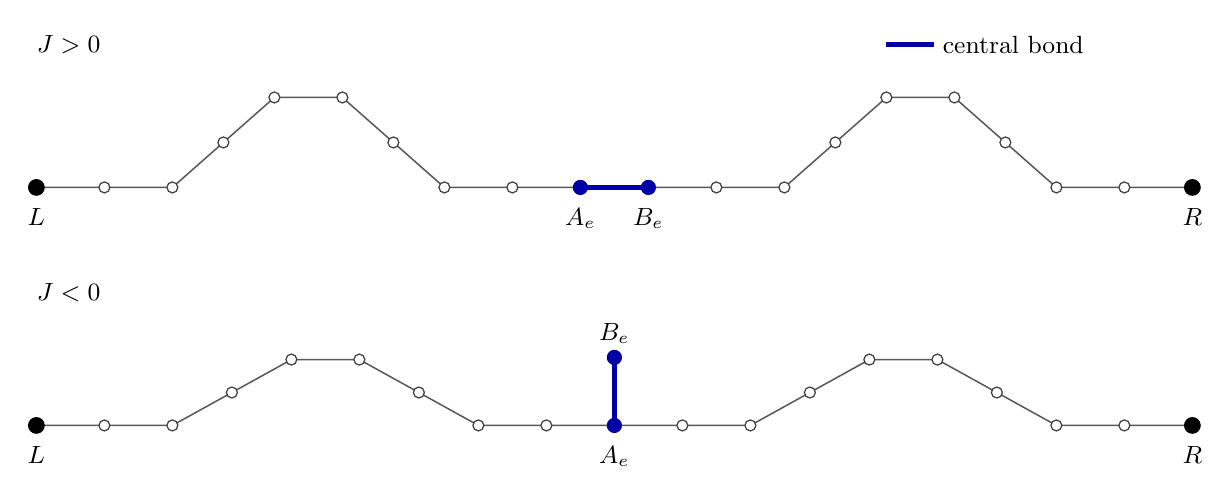
\begin{tikzpicture}[
    x=0.34in,y=0.34in,
    path edge/.style={draw=black!65,line width=0.55pt},
    central edge/.style={draw=blue!65!black,line width=1.6pt},
    site/.style={circle,draw=black!75,fill=white,
      line width=0.45pt,inner sep=1.4pt},
    endpoint/.style={circle,draw=black,fill=black,inner sep=2pt},
    central site/.style={circle,draw=blue!65!black,
      fill=blue!65!black,inner sep=1.8pt},
    every node/.style={font=\small}
  ]
    \pgfmathsetmacro{\positiveHeight}{sqrt(7)/4}
    \pgfmathsetmacro{\positivePeak}{sqrt(7)/2}
    \pgfmathsetmacro{\negativeHeight}{sqrt(15)/8}
    \pgfmathsetmacro{\negativePeak}{sqrt(15)/4}

    \node[anchor=west,inner sep=0pt] at (0,2.1) {$J>0$};
    \draw[central edge] (12.5,2.1) -- (13.2,2.1);
    \node[anchor=west,inner sep=3pt] at (13.2,2.1)
      {central bond};

    \foreach \start in {0,9} {
      \begin{scope}[shift={(\start,0)}]
        \draw[path edge]
          (0,0) -- (1,0) -- (2,0)
          -- (2.75,\positiveHeight) -- (3.5,\positivePeak)
          -- (4.5,\positivePeak) -- (5.25,\positiveHeight)
          -- (6,0) -- (7,0) -- (8,0);
        \foreach \x/\y in {
          0/0,1/0,2/0,2.75/\positiveHeight,3.5/\positivePeak,
          4.5/\positivePeak,5.25/\positiveHeight,6/0,7/0,8/0
        } {
          \node[site] at (\x,\y) {};
        }
      \end{scope}
    }
    \draw[central edge] (8,0) -- (9,0);
    \node[endpoint] at (0,0) {};
    \node[endpoint] at (17,0) {};
    \node[central site] at (8,0) {};
    \node[central site] at (9,0) {};
    \node[anchor=north,inner sep=0pt] at (0,-0.3) {$L$};
    \node[anchor=north,inner sep=0pt] at (8,-0.3) {$A_e$};
    \node[anchor=north,inner sep=0pt] at (9,-0.3) {$B_e$};
    \node[anchor=north,inner sep=0pt] at (17,-0.3) {$R$};

    \begin{scope}[shift={(0,-3.5)}]
      \node[anchor=west,inner sep=0pt] at (0,1.95) {$J<0$};
      \foreach \start in {0,8.5} {
        \begin{scope}[shift={(\start,0)}]
          \draw[path edge]
            (0,0) -- (1,0) -- (2,0)
            -- (2.875,\negativeHeight) -- (3.75,\negativePeak)
            -- (4.75,\negativePeak) -- (5.625,\negativeHeight)
            -- (6.5,0) -- (7.5,0) -- (8.5,0);
          \foreach \x/\y in {
            0/0,1/0,2/0,2.875/\negativeHeight,3.75/\negativePeak,
            4.75/\negativePeak,5.625/\negativeHeight,6.5/0,7.5/0,8.5/0
          } {
            \node[site] at (\x,\y) {};
          }
        \end{scope}
      }
      \draw[central edge] (8.5,0) -- (8.5,1);
      \node[endpoint] at (0,0) {};
      \node[endpoint] at (17,0) {};
      \node[central site] at (8.5,0) {};
      \node[central site] at (8.5,1) {};
      \node[anchor=north,inner sep=0pt] at (0,-0.3) {$L$};
      \node[anchor=north,inner sep=0pt] at (8.5,-0.3) {$A_e$};
      \node[anchor=south,inner sep=0pt] at (8.5,1.2) {$B_e$};
      \node[anchor=north,inner sep=0pt] at (17,-0.3) {$R$};
    \end{scope}
  \end{tikzpicture}
  \caption{The two fixed contact templates, drawn at their actual relative
    coordinates. Every drawn link has length one, and each bent path has
    nine links. The original vertices remain at $L=(0,0)$ and $R=(17,0)$.
    For $J>0$, the central pair is $A_e=(8,0)$, $B_e=(9,0)$ and the paths
    join $L$ to $A_e$ and $B_e$ to $R$. For $J<0$, it is
    $A_e=(8.5,0)$, $B_e=(8.5,1)$ and both paths meet $A_e$.
    Nonlinks are not drawn.}
  \label{fig:contact-templates}
\end{figure}

\section{Localized modes and the finite fermion model}\label{sec:wells}

The positive spin model now fixes the target exchange strengths $K_e$.
This section constructs smooth localized modes and a finite fermion
Hamiltonian whose low-energy spin interaction reproduces $H_+$ up to
scale and a scalar shift. Its occupancy
penalty retains the intersite direct Coulomb coefficients. Computing the
cost of virtual double occupancy determines the required hopping, which
we then obtain by choosing the mode separations.

We work in coordinates \(y=\lambda x=(r,z)\) with \(r\in\mathbb R^2\). The common \(\lambda\) will be polynomially large. After dividing energies by \(\lambda^2\), kinetic energy is the usual \(-\Delta/2\), each unit nucleus has coupling \(1/\lambda\), and electron repulsion has coefficient \(1/\lambda\).

\subsection{Local modes and Coulomb coefficients}\label{subsec:local-modes}

Take \(f(r)=(1-|r|^2)_+^{16}\), and fix
\[
 \phi=(-\Delta_r+1)^{-1}f,\qquad \varphi=\phi/\|\phi\|_2,\qquad
 W(r)=-\frac{f(r)}{2\phi(r)} .
\]
These functions have more bounded continuous derivatives than needed below (in particular through order six). \(W\) is nonpositive and compactly supported, and \(\phi\) is strictly positive, radial, exponentially decaying. For details,
\[
  \phi(r)=\int_0^\infty e^{-t}\int_{\mathbb R^2}
   (4\pi t)^{-1}e^{-|r-b|^2/(4t)} f(b)\,db\,dt
\]
solves the equation by the Gaussian heat kernel identity. For \(|r|>2\), it and the derivatives needed below are bounded in absolute value by \(C(1+|r|)^C e^{-|r|}\), by differentiating on \(f\) and using \(t+(|r|-1)^2/(4t)\ge |r|-1\); for example integrate \(dt/t\) with this bound from 1 to \(|r|^2\), bounding the omitted tails directly by Gaussian or exponential decay. Integrating over \(b\) in the inner half disk and \(|r|/2<t<|r|/2+1\) also gives a lower bound on \(\phi\) of the form \(c(1+|r|)^{-C}e^{-|r|}\).

The isolated planar operator \(-\Delta_r/2+W\) has ground state \(\varphi\), energy \(-1/2\), and a fixed positive gap above that mode. Indeed the shifted form on test functions \(u\) is \(\int \phi^2 |\nabla(u/\phi)|^2/2\); by closure and local positivity this gives nonnegativity and a simple kernel. A unit sequence perpendicular to the kernel with form tending to zero would be bounded in \(H^1\) and, upon extraction, converge weakly and locally in \(L^2\) (strongly on compact sets). By compact support of \(W\) its limit would be in the kernel, hence zero. But then the \(1/2\) shift of the form precludes convergence of the form values to zero. For the transverse direction \(z\) we use the normalized Gaussian \(g(z)=(\omega/\pi)^{1/4}e^{-\omega z^2/2}\) of \(-\partial_z^2/2+2\pi\rho z^2\) with energy \(\omega/2\), \(\omega=\sqrt{4\pi\rho}\), where \(\rho>0\) is a large fixed integer to be chosen. This mode too has a fixed gap (same positive ground-state identity, with compactness here from confinement).

We will place the planar centers \(u_i\) at scale \(D=\log\lambda\) using the contact layout. For all sufficiently accurate implementations, we require minimum spacing \(\ge0.95D\), nonlink spacing \(\ge1.2D\), and extent \(\operatorname{poly}(n) O(D)\). Define
\[
 \begin{gathered}
 \psi_i(y)=\varphi(r-u_i) g(z),\quad e_*=-1/2+\omega/2,\\
 v_{ij}=\iint\frac{\psi_i(y)^2\psi_j(y')^2}{|y-y'|}\,dy\,dy'
       =v(|u_i-u_j|),\qquad U=v(0).
 \end{gathered}
\]
These constants measure direct electron repulsion: $U$ is the same-site
coefficient and $v_{ij}$ the coefficient between sites $i$ and $j$.
They are bounded uniformly. The function \(v\) is radial as indicated
and uniformly Lipschitz, as follows by translating the smooth density
with decaying derivatives.

To control departures from one electron per site, we need a uniform
lower bound on the Coulomb quadratic form. We prove
\((v_{ij})\ge cI\), with fixed \(c>0\), uniformly over these separated
geometries once the polynomial scale is sufficiently large. For real
coefficients \(a_i\), put \(F=\sum_i a_i\psi_i^2\). Choose a fixed
smooth nonnegative, nonzero test bump near the origin, and let
\(\chi_i\) be its disjoint translates to the centers \((u_i,0)\).
With \(w=\sum_i a_i\chi_i\), Poisson's equation and integration by
parts give
\[
 \left|\int Fw\right|^2\le
 \frac1{4\pi}\left(\iint\frac{F(y)F(y')}{|y-y'|}\,dy\,dy'\right)
       \int|\nabla w|^2
\]
for these smooth decaying densities, or first after truncation at
infinity. To bound the left side below even for signed \(a_i\), let
\(A_{ij}=\int\psi_i^2\chi_j\). Its diagonal entries equal a fixed
\(a_*>0\), while the row and column sums of its off-diagonal entries
are exponentially small in \(D\), up to a polynomial factor in \(m\).
Thus \(A=a_*I+R\), with \(\|R\|\le a_*/2\) at our scales, and
\[
       \int Fw=a^{\mathsf T}Aa\ge(a_*/2)\sum_i a_i^2,
       \qquad \int|\nabla w|^2=O\Bigl(\sum_i a_i^2\Bigr).
\]
The displayed Coulomb inequality proves the required lower bound.
Here and below we take \(\lambda\) so large a power of \(n\) that
exponential-in-\(-D\) bounds beat the polynomial factors. In particular,
applying the bound to two sites and coefficients \((1,-1)\) shows that
\(U-v(d)\) is bounded away from zero for every distance
\(d\ge0.95D\) in use; it is also uniformly bounded above.

\subsection{The occupancy penalty and spin exchange}\label{subsec:finite-fermion}

For the moment keep any geometry satisfying the separation bounds, and
let the hopping strengths \(t_e\) be free parameters. On \(2m\)
canonical fermion modes, two spins at each site, restrict to \(m\)
electrons and write \(n_i\) for total occupancy at site \(i\). For
this finite model we multiply dilated energies by \(\lambda\), so
its Coulomb coefficients have no \(1/\lambda\) factor. The direct
Coulomb interaction is
\[
       \frac U2\sum_i n_i(n_i-1)+\sum_{i<j}v_{ij}n_i n_j.
\]
Set \(s_i=\sum_{j\ne i}v_{ij}\). A diagonal one-body term
\(-\sum_i s_i n_i\) cancels the terms linear in the occupancy defects:
using \(v_{ii}=U\) and \(\sum_i n_i=m\),
\begin{equation}\tag{C}\label{eq:occupancy-completion}
 \begin{aligned}
 &\frac U2\sum_i n_i(n_i-1)+\sum_{i<j}v_{ij}n_i n_j-\sum_i s_i n_i\\
 &\hspace{2em}=\frac12\sum_{i,j}v_{ij}(n_i-1)(n_j-1)-\sum_{i<j}v_{ij}.
 \end{aligned}
\end{equation}
Section~\ref{sec:density} will produce this one-body term by adjusting
the well depths. The finite Hamiltonian to be realized is therefore
\[
 \begin{split}
 H_d(t)={}&\frac12\sum_{i,j}v_{ij}(n_i-1)(n_j-1)-\sum_{i<j}v_{ij}\\
    &-\sum_{e=\{i,j\}}t_e
       \sum_{\sigma=\uparrow,\downarrow}
          (c_{i\sigma}^\dagger c_{j\sigma}+c_{j\sigma}^\dagger c_{i\sigma}).
 \end{split}                                                   \tag{2}\label{eq:2}
\]
The nonnegative quadratic penalty has kernel exactly the singly occupied
spin space. It has a fixed gap: a nonzero integer defect vector
\((n_i-1)_i\) has sum zero, hence squared length at least two, so its
penalty is at least \(c\) by Coulomb coercivity.

Hopping vanishes on first-order compression to single occupancy. Its
second-order effect is the double-occupancy superexchange familiar from
Anderson~\cite[Eqs.~(12)--(13), (18)--(21)]{Anderson1959}; his transfer-energy discussion
also retains intersite Coulomb contributions. The normalization and error
bound below are proved for the precise matrix used here.

One allowed hop on \(e=\{i,j\}\) creates a doubly occupied site and
an empty site. Its defect vector is \((1,-1)\) on that pair and zero
elsewhere, so its excitation energy is exactly \(U-v_{ij}\). Only a
hop on the same link can restore single occupancy in one further step.
For hopping strength \(t_e\), the negative second-order operator is
\[
                  \frac{t_e^2}{U-v_{ij}}(h^s_{ij}-I).
\]
Indeed the triplets do not hop into same-site pairs, while the singlet
hops into two orthogonal doubly occupied states with amplitudes of
magnitude \(\sqrt2\,t_e\). Apply the creation and annihilation
operators to
\((c_{i\uparrow}^\dagger c_{j\downarrow}^\dagger-
c_{i\downarrow}^\dagger c_{j\uparrow}^\dagger)|0\rangle/\sqrt2\)
to obtain these amplitudes. Other sites can be placed after these two in
the ordering: changing the ordering of singly occupied sites gives only
an overall sign on the spin space.

With a common positive parameter \(\tau\) to be fixed below, choose
target hoppings
\[
                  t_e^{\rm tar}=\tau\sqrt{K_e(U-v_{ij})}.
\]
They give the effective spin term
\(\tau^2(H_+-\sum_e K_e)\). Their hopping operator has norm at most
\(\tau\operatorname{poly}(n)\), uniformly over admissible separated
geometries. By Lemma~\ref{lem:perturbation}, the energy remainder is at
most \(C\tau^3\operatorname{poly}(n)\), since the penalty gap is
uniform. Fix a rational inverse-polynomial \(\tau>0\) small enough
that the lemma applies and this remainder is at most
\(\gamma\tau^2/100\). This choice is independent of \(\lambda\)
and of the final centers.

\subsection{Calibrating the separations}

The modes supply the hopping profile
\[
 T(d)=-\int_{\mathbb R^2}\varphi(r)W(r)\varphi(r-d e_1)\,dr
     =\frac{1}{2\|\phi\|_2^2}\int f(r)\phi(r-d e_1)\,dr .
\]
It is positive, uniformly Lipschitz, and lies between
\(c(1+d)^{-C}e^{-d}\) and \(C(1+d)^Ce^{-d}\) by the tail
estimates. The continuum compression will supply hopping
\(t_e=\lambda T(|u_i-u_j|)\) in the units of \(H_d\). Although the
occupancy penalty involves every pair, the target hopping on link
\(e\) depends only on its own distance through \(v_{ij}=v(d)\).
Thus each link requires a scalar solve for
\[
           F_e(d)=\lambda T(d)-\tau\sqrt{K_e(U-v(d))}.
\]
At \(d=(1-\varepsilon/2)D\) and \(d=(1+\varepsilon/2)D\),
respectively, \(F_e\) is positive and negative if the fixed polynomial
exponent in \(\lambda\) is sufficiently large. Indeed the first
term has respective sizes \(\lambda^{\varepsilon/2}\) and
\(\lambda^{-\varepsilon/2}\), up to powers of \(D\), whereas the
target has polynomial upper and inverse-polynomial lower bounds in
\(n\).

Bisection with approximate sign tests finds an inverse-polynomially
small residual: stop if the sign is ambiguous within the evaluation
error, or continue until the bracket width times a Lipschitz bound is
small enough. No monotonicity or derivative lower bound is required.
The link-length construction in Section~\ref{sec:spin}, rescaled by
\(D\), then implements all these distances at once. Its contraction
solves and a final rational approximation give rational centers with the
required separations and hopping accuracy. Section~\ref{sec:implementation}
details the numerical evaluation.

From now on, \(H_d\) means \(H_d(t)\) at these final centers with
\(t_e=\lambda T(|u_i-u_j|)\). Choose the per-link calibration accuracy
so that replacing \(t_e^{\rm tar}\) by \(t_e\) changes the total
Hamiltonian norm by at most \(\gamma\tau^2/100\). Together with the
second-order remainder, this gives
\[
  |E(H_d)+\sum_{i<j}v_{ij}
       -\tau^2(E(H_+)-\sum_e K_e)|\le 2\gamma\tau^2/100.       \tag{3}\label{eq:3}
\]

\subsection{Polynomial scale convention}\label{subsec:scales}

Equation~\eqref{eq:3} fixes the finite-model accuracy required of the
continuum construction. All subsequent errors must fit inside an
inverse-polynomial fraction of $\gamma\tau^2$ in the energy units of
$H_d$.

In the estimates below \(p(n,D)\) denotes a polynomial upper bound with uniform coefficients and exponents, which may be enlarged between uses. All requirements of the form "make \(p(n,D)\lambda^{-\alpha}\) small" for fixed \(\alpha>0\), with required smallness at worst inverse polynomial in \(n\), can be imposed simultaneously. Specifically we take an integer \(k\) growing as a sufficiently large fixed power of \(n\) (allowing a fixed factor) and put
\[
                  h=1/k,\qquad \lambda=8k^3/\rho .
\]
Here \(h\) will be the side length of the cubature cells in
Section~\ref{sec:nuclei}; the relation
\(\rho h^3/8=1/\lambda\) gives each of their eight nodes the mass
needed for a unit nucleus. Other magnitudes such as the large box used
below will have stated polynomial bounds in \(\lambda,n\); its volume
will enter \(p(n,D)\) only when explicitly accounted for. The fixed
\(\rho\) only has to dominate bounded potential derivatives as described
next and can be chosen before these scale choices.

\section{Synthesis by a nonnegative charge density}\label{sec:density}

We now construct an attractive Coulomb potential whose low-energy
matrix realizes the modes and hopping of Section~\ref{sec:wells}.
A broad slab supplies the transverse oscillator near the modes and a
positive background density. Adding the planar wells then changes the
density by a bounded, compactly supported term, so the total density
remains nonnegative. We first construct this potential, then establish
a fixed energy cost outside the mode space and compute its matrix on
that space.

\subsection{The slab and the well-depth counterterm}

Use integers \(S\) of size between \(D\) and \(10D\), and \(H=\lceil\lambda^5\rceil\). (For \(S\) one can use a binary bit-length scale.) Let
\[
 \Omega=[-H,H]^2\times[-S,S],\qquad
 F_H(y)=-\rho\int_\Omega\frac{db}{|y-b|},\qquad C_H=F_H(0).
\]
The occupancy identity~\eqref{eq:occupancy-completion} requires the
one-body diagonal \(-s_i/\lambda\), where
\(s_i=\sum_{j\ne i}v_{ij}\). Put \(W_i=W(\,\cdot-u_i)\).
Since \(\langle\psi_i,W_i\psi_i\rangle=\int\varphi^2W<0\),
a small increase in each well depth has the required sign and size.
Take a fixed sufficiently smooth cutoff \(\zeta\) between 0 and 1,
supported inside \((-1,1)\), equal to 1 for \(|z|\le 1/2\);
it may be piecewise polynomial with rational data. Define
\[
 b_i=\frac{s_i}{-\int\varphi^2 W},\qquad
 V_\ell(r,z)=\zeta(z/S)\sum_i(1+b_i/\lambda)W_i(r).
\]
These \(b_i\ge0\) are polynomially bounded independent of \(D\); hence \(0\le b_i/\lambda<1\) at our scales. For all \(S\ge1\) the derivatives we need of \(V_\ell\) are bounded independently, by disjoint planar supports. Choose the fixed integer \(\rho\) so large, using \(1+b_i/\lambda\le2\), that \(|\Delta V_\ell/(4\pi)|\le\rho/2\). There is no circularity, since the bound based on \(2,W,\zeta\) does not depend on the vertical Gaussian or \(b_i\). The centers fit well inside the horizontal box for our scale. Thus
\[
               F_H+V_\ell
   =-\int_\Omega \frac{\rho+\Delta V_\ell(b)/(4\pi)}{|y-b|}\,db       \tag{4}\label{eq:4}
\]
by compact support and the fundamental solution identity.

Thus the density in~\eqref{eq:4} lies between \(\rho/2\) and
\(3\rho/2\) on \(\Omega\). Its total mass is \(\rho|\Omega|\),
because \(\int\Delta V_\ell=0\). The next estimates show that the
truncated slab approximates the harmonic potential near the modes and
provides a global lower bound outside that region.

Here are useful background estimates with constants independent of \(n,\lambda\):
\[
 \begin{split}
 F_H(y)-C_H &\ge 2\pi\rho \min(z^2,S^2)- C S^3/H,\\
 |F_H(y)-C_H-2\pi\rho z^2|
      &\le C(S^3+S|r|^2)/H
           \qquad (|r|\le H/2,\ |z|\le S).
 \end{split}                                                       \tag{5}\label{eq:5}
\]
Indeed \(F_H\) at each \(z\) is minimized at \(r=0\), and is also nondecreasing in \(|z|\) for fixed \(r\). These statements follow one coordinate at a time by integration of even decreasing kernels on centered intervals. At \(r=0\), extending the horizontal integration to the plane in the difference between \(z\) and 0 gives for \(|z|\le S\) exactly \(2\pi\rho\int_{-S}^S(|z-w|-|w|)\,dw=2\pi\rho z^2\), by polar integration. The omitted difference costs \(CS^3/H\), by inverse cube decay outside horizontal radius \(H\). For \(|r|\le H/2\), the change relative to the horizontal center is bounded by \(CS|r|^2/H\). For example translate the integration square instead of translating the kernel. The first derivatives then come from sides at distance at least \(H/2\), and second derivatives are bounded by \(CS/H\) by integrating first derivatives of the kernel on the sides. Evenness at zero gives the bound. Finally \(0\ge F_H(y)\ge C_H\) and \(|C_H|\le CSH\).

\subsection{The one-particle gap and residual}

The potential has now been expressed as the Coulomb field of a
nonnegative density. Before replacing it by point nuclei we need two
properties: a fixed energy gap outside the prescribed modes, and a small
residual on those modes. The gap will control arbitrary continuum
states, while the residual will control mixing with the mode space.

Let the shifted continuous one-particle operator, still before point-charge replacement, be
\[
       L_c=-\Delta_y/2+F_H+V_\ell-C_H-e_* .
\]
We suppress the tensor identity on spin. Let \(P\) project onto the span
of the \(\psi_i\), including both spins when present, and write
\(\Gamma_{ij}=\langle\psi_i,\psi_j\rangle\) for their spatial Gram
matrix. Exponential tails and the \(0.95D\) spacing give
\(\|\Gamma-I\|\le p(n,D)\lambda^{-0.8}\): for example, each
off-diagonal overlap is \(O(e^{-0.9|u_i-u_j|})\), by leaving part of
the decay as an integrable factor. We use the orthonormal modes
\[
 \widehat\psi_j=\sum_i\psi_i(\Gamma^{-1/2})_{ij},\qquad
 \|\Gamma^{-1/2}-I\|\le p(n,D)\lambda^{-0.8}.
\]
In particular, unit vectors in \(\operatorname{Ran}P\) have
polynomially bounded one-particle kinetic energy.

\begin{proposition}[Continuous one-particle control]\label{prop:continuous-control}
For the density and separated centers constructed above, with the
polynomial scale chosen sufficiently large, there are fixed constants
\(c>0,C<\infty\) such that
\[
 \begin{split}
 (I-P)L_c(I-P)&\ge c(I-P)\quad\text{on the complement},\\
 L_c&\ge -\Delta_y/2-C,\qquad
 \|L_cP\|\le p(n,D)\lambda^{-0.9}.
 \end{split}                                                       \tag{6}\label{eq:6}
\]
The inequalities are quadratic-form inequalities on the one-particle
$H^1$ domain, and the last bound is an operator norm from the range of
$P$ to $L^2$. All estimates hold with either spin included.
\end{proposition}

\begin{proof}
For the first inequality compare below, using \eqref{eq:5}, with the separable planar multiwell \(-\Delta_r/2+\sum W_i\) plus the vertical operator with capped potential \(2\pi\rho\min(z^2,S^2)\), shifted by \(-e_*\). Errors in the lower bound are \(O(S^3/H)+O(p(n,D)/\lambda)\), since \(\zeta W_i\ge W_i\) and the \(b_i/\lambda\) terms are small and bounded everywhere. 

For clarity we detail the gap argument. In the plane use a quadratic partition of unity consisting of cutoffs about each site (equal to one inside radius \(D/8\), supported at radius \(D/3\)) and a remaining exterior function. They can be built by smooth angle interpolation from 0 to \(\pi/2\) on the transition annuli using sine and cosine, with squared gradients summing to \(C/D^2\) or less. The localization form identity (IMS localization; compare
\cite[Lemma 3.1]{Simon1983}), obtained here by the product rule with
kinetic coefficient $1/2$, then costs \(O(1/D^2)\). In each site term use the isolated ground and gap bound, and in the exterior use the free kinetic lower bound. This gives
\[
 -\Delta_r/2+\sum W_i \ \ge\
 -1/2+c_1(I-P_r)-o(1)I,
\]
where \(P_r\) projects on the planar translates of \(\varphi\), \(c_1>0\) can be taken below the isolated gap and \(1/2\), and the small bound can be made uniformly small. In detail, with site cutoffs \(\theta_i\) and \(\varphi_i=\varphi(\cdot-u_i)\), the site term evaluated on \(\theta_i u\) is at least
\[
 (-1/2+c_1)\|\theta_i u\|^2-c_1|\langle\theta_i\varphi_i,u\rangle|^2;
\]
the exterior term also bounds its share of the \(-1/2+c_1\) term as there is no well on its support. The sum of rank-one operators from the cutoff ground-state modes differs from \(P_r\) by at most \(O(m e^{-c' D})+O(p(n,D)\lambda^{-0.8})\), by the tails and Gram bound. 

Similarly localize the vertical problem with an inner cutoff equal to one on \(|z|\le S/2\), supported on \(|z|\le S\), and an exterior function. Use the harmonic gap and the large \(z\) potential lower bound on the respective terms, at gradient cost \(O(S^{-2})\), with Gaussian loss on the rank-one mode. This gives a vertical lower bound \(\omega/2+c_2(I-P_g)-o(1)I\), where \(P_g=|g\rangle\langle g|\). Since \(P=P_r\otimes P_g\) on the spatial space and
\[
 (I-P_r)\otimes I+I\otimes(I-P_g)\ge I-P,
\]
the tensor sum has a fixed gap on \(I-P\) once the errors are small.

The slowly small errors such as \(O(D^{-2})\) here are needed only for a fixed gap estimate, not as the energy accuracy per particle.

The kinetic lower bound in \eqref{eq:6} follows from \eqref{eq:5} or background minimality and bounded \(V_\ell\). For the residual estimate, \eqref{eq:5}, the crude global background bound, and the mode tails give
\[
  \|(F_H-C_H-2\pi\rho z^2)\psi_i\|_2\le p(n,D)\lambda^{-2}.
\]
Indeed moments with \(|r|\le H/2,\ |z|\le S\) suffice there, and outside this region the Gaussian or planar exponential beats the global polynomial magnitudes, using \(S\ge\log\lambda\). The cutoff defect in \(V_\ell\) versus \(\sum_i(1+b_i/\lambda)W_i\) acting on any mode is likewise negligible. Since \((-{\Delta_y}/2+2\pi\rho z^2+W_j-e_*)\psi_j=0\), the remaining residual is a sum of other wells acting on the small planar tails and the term with \(b_j/\lambda\). This proves \eqref{eq:6}.
\end{proof}

\subsection{The compressed one-particle matrix}

The fixed complementary gap alone does not give the required energy
accuracy. We therefore compute the matrix on the prescribed modes,
including its diagonal counterterm, to a sharper scale.

The continuous one-body compression can now be evaluated more precisely. On the nonorthogonal functions before Gram correction, the column on mode \(j\) comes, up to background and cutoff errors as above, from
\[
                  \Big(\sum_{k\ne j} W_k+\lambda^{-1}\sum_k b_k W_k\Big)\psi_j .
\]


On row \(j\), the leading contribution is \(-\lambda^{-1}\sum_{i\ne j}v_{ij}\) by construction; the other-well integrals there use two tail factors. On row \(i\ne j\) the first sum at \(k=i\) gives \(-T(|u_i-u_j|)\). The cases \(k\ne i,j\) of the first sum are products of two tail factors at a third site; each such integral is \(O(\lambda^{-1.8})\) by the spacing and compact well support. Terms with the explicit \(\lambda^{-1}\) give only negligible off-diagonal errors (at least one planar tail on each well support, hence bounded by \(p(n,D)\lambda^{-1.9}\) altogether on such an entry). Nonlink hoppings cost at most \(p(n,D)\lambda^{-1.2}\) per term. 

To pass to the orthonormal modes, let
\(A_{ij}=\langle\psi_i,L_c\psi_j\rangle\). The matrix becomes
\(\Gamma^{-1/2}A\Gamma^{-1/2}\), and
\[
 \|\Gamma^{-1/2}A\Gamma^{-1/2}-A\|
 \le C\|\Gamma-I\|\,\|A\|
 \le p(n,D)\lambda^{-1.7}
\]
by~\eqref{eq:6}. Here \(A\) is the \emph{shifted} matrix: subtracting
\(C_H+e_*\) before making this estimate removes the large background
scalar. The correction therefore remains negligible after
multiplication by \(\lambda\).

Define the spatial matrix
\[
 \mathsf M_{ij}=\begin{cases}
  -s_i,&i=j,\\
  -\lambda T(|u_i-u_j|),&\{i,j\}\text{ is a link},\\
  0,&\text{otherwise}.
 \end{cases}
\]
The preceding estimates give
\[
 \bigl\|\lambda\Gamma^{-1/2}A\Gamma^{-1/2}-\mathsf M\bigr\|
       \le p(n,D)\lambda^{-0.1}.
\]
This is the required one-particle compression, with the identity on
spin. The diagonal supplies the depth counterterm, and the link
entries supply the calibrated hopping.

\section{Replacing the density by unit nuclei}\label{sec:nuclei}

Our input is the nonnegative density in~\eqref{eq:4}. We must replace its
Coulomb field by finitely many equal masses $1/\lambda$, so that physical
nuclear charges are all one. The construction has two distinct error
requirements: a form bound on arbitrary states and a stronger
compression bound on the smooth localized modes.

The comparison with \(H_d\) uses energies multiplied by \(\lambda\).
A compressed error must therefore be smaller than \(\lambda^{-1}\),
up to the required polynomial margin. The error coupling the mode space
to its complement can be larger: the fixed complementary gap makes its
energy contribution quadratic, as proved in
Section~\ref{subsec:complement-control}. With
\(h=(8/(\rho\lambda))^{1/3}\), a cubature rule exact through degree
three will give an \(O(h^4)\) compressed error and an \(O(h^2)\) form
error. Both resulting energy errors are \(O(\lambda^{-1/3})\) in
the units of \(H_d\), up to polynomial factors.

\subsection{Transport and charge placement}\label{subsec:charge-placement}

The density interpolation uses Moser's deformation
method~\cite[Section 4]{Moser1965}, also developed by Dacorogna and
Moser~\cite[Section II, Lemma 3]{DacorognaMoser1990}. Here the vector
field is explicit and compactly supported inside the box; the following
continuity-equation calculation proves the required transport directly.
Write
\(q_t=\rho+t\Delta V_\ell/(4\pi)\), so that \(q_0=\rho\)
and \(q_1\) is the desired density on \(\Omega\). Since
\(q_t\ge\rho/2\), the time-dependent vector field on full space
\[
 \mathcal V_t(b)=-\frac{\nabla V_\ell(b)}{4\pi q_t(b)},
 \qquad 0\le t\le1,
\]
has uniformly bounded derivatives through order four. It vanishes
outside the well cylinders strictly inside the box. Let \(G_t\) be its
flow from time zero and put \(G=G_1\). The ODE and its differentiated
equations give bounded derivatives of \(G\) through order four and a
bounded Lipschitz inverse. The flow is the identity off the cylinders
and preserves \(\Omega\).

The identity \(\partial_t q_t+\nabla\cdot(q_t\mathcal V_t)=0\)
gives
\[
 q_t(G_t(b))\det DG_t(b)=\rho,\qquad
 \int_\Omega F(b)q_1(b)\,db
       =\rho\int_\Omega F(G(b))\,db.
\]
Thus the flow transports the uniform measure to the target density.
The last formula also shows how to retain equal cubature masses:
move the nodes by \(G\) and keep their weights unchanged.

Since \(H,S,k\) are integers, cubes of side \(h=1/k\) tile
\(\Omega\). On each cube use the eight tensor products of the two
equal-weight Gauss points per coordinate, at the midpoint plus or minus
\(h/(2\sqrt3)\). The rule integrates polynomials of total degree at
most three exactly, by the corresponding moments on each interval.
Map these nodes by \(G\). Their common mass remains
\(\rho h^3/8=1/\lambda\); polynomial exactness is used in the
original cube coordinates, on integrands composed with \(G\).

Each exact mapped point \(b_\alpha\) will be approximated within
Euclidean error at most
\[
                    \delta_R\le (1+H)^{-3}(1+S)^{-2}\lambda^{-3}
\]
by rational points \(\tilde b_\alpha\), and the physical nuclear positions are \(\tilde b_\alpha/\lambda\). They remain distinct by node separation and bi-Lipschitz bounds.

\subsection{Form and compression estimates}\label{subsec:nuclear-errors}

Let \(L_p\) be the shifted one-particle operator with these actual point nuclei in dilated units, i.e. with potential \(-\sum_\alpha \lambda^{-1}/|y-\tilde b_\alpha|-C_H-e_*\). \begin{proposition}[Unit-nucleus replacement]\label{prop:nuclear-replacement}
For the transported degree-three cubature and rational rounding just
specified, with $\delta_R\le(1+H)^{-3}(1+S)^{-2}\lambda^{-3}$, the
shifted continuous and point-nucleus operators $L_c,L_p$ satisfy
\[
 \begin{split}
 |\langle u,(L_p-L_c)u\rangle|
      &\le p(n,D)\lambda^{-2/3}(\|u\|^2+\|\nabla u\|^2),\\
 \|P(L_p-L_c)P\|_{P}
      &\le p(n,D)\lambda^{-4/3}.
 \end{split}                                               \tag{7}\label{eq:7}
\]
The first estimate holds for every one-particle $H^1$ function $u$.
The second is the norm of the compressed form on the localized-mode
space $\operatorname{Ran}P$. Both bounds are in dilated energy units.
\end{proposition}

\begin{proof}
We first work at the exact transported nodes. On an original grid cube
\(Q\), write \(a_{Q,\nu}\), \(1\le\nu\le8\), for its Gauss
nodes. Taylor's theorem and exactness through degree three give the
common error estimate
\[
 \left|\rho\int_Q F(G(b))\,db
   -\frac{\rho h^3}{8}\sum_{\nu=1}^8 F(G(a_{Q,\nu}))\right|
 \le C h^7\sup_Q |D^4(F\circ G)|
\]
whenever \(F\circ G\) has four bounded derivatives on \(Q\).
We apply this first to the singular Coulomb kernel away from its
singularity, then to the smooth fields obtained after compression.

\noindent\textbf{General form estimate.} For fixed evaluation point \(y\), the charge integral is of the kernel \(|y-G(b)|^{-1}\) against uniform density in \(b\). For cubes whose images touch a ball of radius a fixed large constant times \(h\) about \(y\), there are only \(O(1)\) such cubes. Their continuous contribution is \(O(h^2)\) by bounded transformed density. The discrete one is bounded by a sum of \(C h^3/|y-b_\alpha|\) with \(|y-b_\alpha|\le C'h\). 

On farther cubes, the pure fourth derivative of the kernel is bounded
by \(C|y-G(b)|^{-5}\). Distances to \(y\) are comparable within
each such cube, and the bi-Lipschitz change of variables has bounded
Jacobian. Summing the pure derivative contributions therefore costs
at most
\[
 C h^4\int_{|x-y|>ch}|x-y|^{-5}\,dx=O(h^2).
\]
The other chain-rule terms contain a derivative of \(G\) of order
at least two and a kernel derivative bounded by
\(C|y-G(b)|^{-j}\), \(2\le j\le4\). Such terms occur only on
cells meeting the well cylinders, of combined volume
\(O(m(S+1))\). Below distance one they are bounded by the same
inverse fifth power; beyond distance one their contribution is at
most \(C h^4m(S+1)\).

This proves a pointwise absolute error bound by \(C(h^2+h^4 m(S+1))\) plus the close-node sum above. In particular there is no factor the size of the large horizontal area in this bound.

The close-node balls have bounded overlap also upon any fixed dilation. Around each node one has
\[
  \int_{|y-b_\alpha|\le C'h}\frac{|u(y)|^2}{|y-b_\alpha|}\,dy
  \le C\int_{|y-b_\alpha|\le 2C'h}
                       (h^{-1}|u|^2+h|\nabla u|^2).
\]
This follows by a cutoff and the three-dimensional Hardy inequality \(\int |u|^2/|y|^2\le4\int|\nabla u|^2\), which follows also by the divergence formula for \(y/|y|^2\) and Cauchy-Schwarz. Summing gives the general form bound, since \(h^2=O(\lambda^{-2/3})\).

\noindent\textbf{Compressed estimate.} For compression use the smooth Coulomb fields
\[
     K_{ij}(b)=\int |y-b|^{-1}\psi_i(y)\psi_j(y)\,dy .
\]
Their derivatives through order four are uniformly bounded (differentiate the translated densities). Fourth derivatives satisfy
\[
         |D_b^4 K_{ij}(b)|\le C(1+|b-(u_i,0)|)^{-5}.
\]
Indeed derivatives of the product density decay exponentially about \((u_i,0)\), uniformly by bounded derivatives on the other factor. At a large distance \(d=|b-(u_i,0)|\), use a smooth density cutoff supported within distance \(d/2\) of that center and equal to one inside \(d/3\), with the cutoff radius held fixed when differentiating. There one uses pure kernel derivative decay, and on the remaining tail one differentiates the cut-off density instead, with exponentially small bounds. This proves the assertion. Applying the same degree-three cubature to \(K_{ij}\circ G\) now costs \(O(h^4(1+m(S+1)))\) for each entry: pure fourth derivatives have summable volume bounds as just proved, and other chain-rule terms live on the exceptional cells. Gram correction and taking matrix norms cost at most polynomial factors. This proves the second estimate for exact nodes.

\noindent\textbf{Rounding.} A center shift of size \(\delta_R\)
changes the inverse distance by at most
\(\delta_R/(|y-b_\alpha|\,|y-\tilde b_\alpha|)\).
Cauchy--Schwarz and translated Hardy inequalities bound its form
by \(4\delta_R\|\nabla u\|^2\). Summing the masses gives the
total bound \(4\rho|\Omega|\delta_R\|\nabla u\|^2\), where
\[
 \rho|\Omega|\delta_R
 \le C H^{-1}S^{-1}\lambda^{-3}
 \le C\lambda^{-8}.
\]
This is smaller than both required errors, also after compression
because the modes have polynomial kinetic bounds. It completes
\eqref{eq:7}.
\end{proof}

We have obtained the two replacement estimates with constants
independent of the horizontal area of the slab. The full mass enters
only the rounding bound, where the chosen coordinate accuracy absorbs
it. Section~\ref{sec:many-body} now combines these estimates with the
fixed complementary gap and the compressed matrix from
Section~\ref{sec:density}.

\section{Many-electron continuum estimate}\label{sec:many-body}

The point nuclei have now been fixed. We must compare their electronic
energy with the finite Hamiltonian $H_d$ on \emph{all} continuum states.
First we eliminate the space in which some electron lies outside the
localized modes, using the fixed gap and the two replacement estimates.
Then we identify the compressed Hamiltonian, keeping direct Coulomb
repulsion exactly at its leading order.

In the dilated coordinates the full operator after dividing by \(\lambda^2\) and shifting by \(-m(C_H+e_*)\) is
\[
             \mathcal H=\sum_{\ell=1}^m (L_p)_\ell+\lambda^{-1}\mathcal R,
           \qquad \mathcal R=\sum_{\ell<s}|y_\ell-y_s|^{-1}.
\]
We work on the antisymmetric space with spins and its $H^1$ form domain.
The Coulomb forms used here have the variational meaning specified in
Section~\ref{sec:introduction}, whether or not their energy infima are
attained. Indeed, fiberwise Hardy and Cauchy--Schwarz give, for every
$\eta>0$ and every fixed center $b$,
\[
 \int\frac{|u|^2}{|y_\ell-b|}
 \le 2\|u\|_2\|\nabla_\ell u\|_2
 \le \eta\|\nabla_\ell u\|_2^2+\eta^{-1}\|u\|_2^2.
\]
The same estimate applies to a pair singularity by fixing the other
coordinates. For each finite nuclear configuration, summing with
sufficiently small $\eta$ gives a closed lower-bounded form whose shifted
form norm is equivalent to the $H^1$ norm. Smooth compactly supported
antisymmetric functions form a core. The spectral infimum is therefore
the infimum of the form over normalized $H^1$ states, and the form
estimates below extend from this core by continuity.

Let $\Pi$ project onto the space in which all $m$ particles lie in $P$,
and write
\[
 \|u\|_1^2=\|u\|^2+\sum_\ell\|\nabla_\ell u\|^2.
\]
The smooth decaying modes lie in the form domain, so their compression is
well defined. The one-particle kinetic bound gives
$\|w\|_1\le p(n,D)\|w\|$ for $w\in\operatorname{Ran}\Pi$.

Let
\[
 E_\Pi=\min\operatorname{spec}
       \bigl((\Pi\mathcal H\Pi)|_{\operatorname{Ran}\Pi}\bigr),
\]
where the compression is defined by the form. This is a finite-dimensional
minimum because $\Pi$ projects onto the $m$-electron space built from
$2m$ one-particle spin modes.

\subsection{Control outside the orbital space}\label{subsec:complement-control}

\begin{proposition}[Eliminating the continuum complement]\label{prop:complement}
For the unit-nucleus construction above with $N=m$, and sufficiently
large polynomial scale $\lambda$, the full antisymmetric $m$-electron
operator in dilated and shifted units satisfies
\[
                 E_\Pi-p(n,D)\lambda^{-4/3}
                   \ \le\ \inf\operatorname{Spec}\mathcal H\ \le\ E_\Pi.       \tag{8}\label{eq:8}
\]
The lower bound holds on every normalized antisymmetric $H^1$ state,
including every spin sector.
\end{proposition}

\begin{proof}
The proof needs a lower bound on the complementary space, a bound on
its coupling to $\operatorname{Ran}\Pi$, and then a square completion.
Write $\mathcal H_c^0=\sum_\ell (L_c)_\ell$. By~\eqref{eq:6}, as
one-particle forms,
\[
                L_c\ge c'(I-P)-p(n,D)\lambda^{-0.9} I
\]
for some $c'>0$: the diagonal and cross terms involving $P$ are
controlled by $\|L_cP\|$. Since
$\sum_\ell(I-P)_\ell\ge I-\Pi$, summing gives a fixed positive lower
bound for $\mathcal H_c^0$ on $\operatorname{Ran}(I-\Pi)$ once
$m p(n,D)\lambda^{-0.9}$ is small. We also have the kinetic lower bound
$\mathcal H_c^0\ge-\sum_\ell\Delta_\ell/2-Cm$. A convex combination,
with a sufficiently small weight of order $1/m$ on the kinetic bound,
retains a positive $L^2$ term and gives
\[
                 \langle q,\mathcal H_c^0 q\rangle
                    \ge (c''/m)\|q\|_1^2,\qquad c''>0,
\]
for $q\in\operatorname{Ran}(I-\Pi)$. By~\eqref{eq:7} on each
coordinate and positivity of $\mathcal R$, this estimate persists with
half that coefficient for $\mathcal H$.

For $w\in\operatorname{Ran}\Pi$, equation~\eqref{eq:6} gives
$\|\mathcal H_c^0w\|\le p(n,D)\lambda^{-0.9}\|w\|$.
Hardy applied with one particle coordinate at a time also gives
$\|\mathcal Rw\|\le p(n,D)\|w\|$. Finally, polarizing the form
bound in~\eqref{eq:7} and using the $H^1$ bound on $w$ controls the
point-nucleus replacement in the mixed block. Together these estimates
give
\[
               |\langle q,\mathcal H w\rangle|
                  \le p(n,D)\lambda^{-2/3}\|w\|\|q\|_1.
\]
The same estimates show that the compressed form has norm less than
$c''/(4m)$ at sufficiently large scale. Set
$\alpha=c''/(4m)$ and let $\beta=p(n,D)\lambda^{-2/3}$ bound the
mixed block. Decompose any normalized form-domain vector as $u=w+q$,
where $w=\Pi u$ and $q=(I-\Pi)u$. Subtracting $E_\Pi$ makes the
$w$-diagonal form nonnegative and leaves at least
$\alpha\|q\|_1^2$ on the complement. Hence, with all pairings
interpreted as forms,
\[
 \begin{split}
 \langle u,\mathcal H u\rangle-E_\Pi\|u\|^2
 &\ge \alpha\|q\|_1^2-2\beta\|w\|\|q\|_1\\
 &\ge -\frac{\beta^2}{\alpha}\|w\|^2
 \ge -p(n,D)\lambda^{-4/3}.
 \end{split}
\]
This proves the lower bound in~\eqref{eq:8}; the upper bound follows by
testing a minimizing vector in $\operatorname{Ran}\Pi$. The lower-bound
argument applies to every normalized antisymmetric state, in any spin
sector, without any binding or ground-eigenvector assumption.
\end{proof}

\subsection{Compressed energy}\label{subsec:compressed-energy}

It remains to evaluate $\lambda E_\Pi$. Section~\ref{sec:density}
computed the one-particle matrix $\mathsf M$ in the orthonormal modes
$\widehat\psi_i$, to accuracy $p(n,D)\lambda^{-0.1}$. Multiplying the
compressed replacement error in~\eqref{eq:7} by $\lambda$ costs only
$p(n,D)\lambda^{-1/3}$, so the same matrix accuracy holds for the
point nuclei.
For the repulsion $\mathcal R$, the pair matrix on the original modes
before Gram correction has spatial entries from products of two
transition densities. Keeping only $\psi_i^2,\psi_j^2$ as the
respective densities gives the direct coefficients $v_{ij}$.
Any unequal indices within a density give an exponentially small error:
$\|\psi_i\psi_k\|_{L^1}=O(\lambda^{-0.8})$ for $i\ne k$, and the
Coulomb field of the other density product in absolute value is
uniformly bounded by orbital boundedness and decay. The matrix of
direct interactions in the product basis is bounded, and Gram
correction changes its entries negligibly.

These entrywise estimates give a many-electron operator-norm error of
at most $p(n,D)\lambda^{-0.1}$. To see the dimension dependence,
write the one- and two-body matrices in the $2m$ orthonormal spin modes.
Each coefficient multiplies a monomial $c_a^\dagger c_b$ or
$c_a^\dagger c_b^\dagger c_d c_c$, of norm at most one. There are
only $O(m^2)$ and $O(m^4)$ such monomials, respectively, so summing their
coefficient errors costs a polynomial factor on the entire fermion
space. In this representation, the retained two-body term is
\[
       \frac{U}{2}\sum_i n_i(n_i-1)+\sum_{i<j}v_{ij} n_i n_j .
\]
The retained one-body diagonal is
$-\sum_i(\sum_{j\ne i}v_{ij})n_i$. At the filling
$\sum_i n_i=m$, the identity~\eqref{eq:occupancy-completion} combines
these terms into the first line of~\eqref{eq:2}, including its scalar.
The hopping matrix gives the remaining line of the calibrated $H_d$.
We have thus identified the compressed Hamiltonian, and the comparison
with the full continuum follows.

\begin{proposition}[Continuum-to-fermion energy comparison]\label{prop:energy-comparison}
For the constructed unit nuclei with $N=m$, let $\mathcal H$ be the
dilated and shifted continuum operator above and let $H_d$ be the
finite fermion Hamiltonian~\eqref{eq:2}. At sufficiently large polynomial
scale,
\[
          |\lambda\inf\operatorname{Spec}\mathcal H-E(H_d)|
                              \le p(n,D)\lambda^{-0.1}.             \tag{9}\label{eq:9}
\]
\end{proposition}

\begin{proof}
The one- and two-body matrix estimates just obtained compare
$\lambda E_\Pi$ with $E(H_d)$ within $p(n,D)\lambda^{-0.1}$.
Multiplying~\eqref{eq:8} by $\lambda$ contributes only
$p(n,D)\lambda^{-1/3}$, which fits within that bound.
\end{proof}
This analysis treats long-range diagonal effects and possible charge transfer at the virtual-excitation scale in \eqref{eq:2}-\eqref{eq:3}, rather than requiring all intersite Coulomb matrix elements to be negligible compared to the input promise gap.

Table~\ref{tab:error-scales} records the different roles of the errors.
In particular the arbitrary-state form error cannot be used as a direct
energy error after multiplication by $\lambda$.

\begin{table}[tbp]
\centering
\small
\begin{tabular}{@{}p{.43\linewidth}p{.18\linewidth}p{.30\linewidth}@{}}
\toprule
Estimate & Error scale & Role in the comparison \\
\midrule
General form replacement, \eqref{eq:7}
 & $\lambda^{-2/3}$ & Controls mixed blocks in the $H^1$ norm \\
Compressed replacement, \eqref{eq:7}
 & $\lambda^{-4/3}$ & Direct error on the mode space \\
Complement elimination, \eqref{eq:8}
 & $\lambda^{-4/3}$ & Square of the mixed-block scale \\
Last two errors after multiplication by $\lambda$
 & $\lambda^{-1/3}$ & Error in the units of $H_d$ \\
Total comparison, \eqref{eq:9}
 & $\lambda^{-0.1}$ & Includes the other mode-matrix errors \\
\bottomrule
\end{tabular}
\caption{Error scales up to polynomial factors $p(n,D)$. The first three
rows use the units of $\mathcal H$; the last two use the units of $H_d$.
The $O(D^{-2})$ and $O(S^{-2})$ localization losses establish a fixed
complementary gap and do not enter the energy-precision budget.}
\label{tab:error-scales}
\end{table}

\subsection{Physical energies and thresholds}\label{subsec:physical-thresholds}

Choose the polynomial scale in $\lambda$ large enough that~\eqref{eq:9}
costs at most $\tau^2\gamma/100$ and that $\lambda\tau^2\gamma\ge8$.
All earlier smallness, separation, and calibration estimates hold
simultaneously by the stated growth choices. Undoing the dilation and
scalar shift gives the physical energy exactly as
\[
 E_0=\lambda^2\left[m(C_H+e_*)+
                         \inf\operatorname{Spec}\mathcal H\right].
\]
Combining~\eqref{eq:1}, \eqref{eq:3}, and~\eqref{eq:9} now gives a
total error at most $7\lambda\tau^2\gamma/100$, and hence at most
$\lambda\tau^2\gamma/8$, from
\[
       \mathcal F(E(H_{\rm in})),\qquad
       \mathcal F(\xi)=
           \lambda^2 m(C_H+e_*)+
           \lambda\left[-\sum_{i<j}v_{ij}
                    +\tau^2\left(\xi-C_s-\sum_e K_e\right)\right].            \tag{10}\label{eq:10}
\]
Take output thresholds rationally approximating \(\mathcal F(a_s+\gamma/4)\) and \(\mathcal F(b_s-\gamma/4)\) each within \(\lambda\tau^2\gamma/32\). For a YES source instance,
\[
 E_0\le\mathcal F(a_s)+\lambda\tau^2\gamma/8
       <\mathcal F(a_s+\gamma/4)-\lambda\tau^2\gamma/32\le a.
\]
For a NO source instance, the reversed estimate gives
\[
 E_0\ge\mathcal F(b_s)-\lambda\tau^2\gamma/8
       >\mathcal F(b_s-\gamma/4)+\lambda\tau^2\gamma/32\ge b.
\]
Since $b_s-a_s\ge\gamma$, the threshold separation satisfies
\[
 b-a\ge\lambda\tau^2\bigl(b_s-a_s-\gamma/2\bigr)
                   -\lambda\tau^2\gamma/16
      \ge\frac7{16}\lambda\tau^2\gamma\ge\frac72>1.
\]
Thus both promises survive rational rounding, and the reduction meets
the required output separation \(b-a\ge1\).

\section{Implementability and encoding}\label{sec:implementation}

The preceding construction specifies the nuclear configuration, and
Section~\ref{subsec:physical-thresholds} gives threshold accuracies
that preserve the source promise. It remains to compute those outputs
in deterministic polynomial time. We first fix the order of the scales,
then explain how to evaluate the orbital integrals and transported nodes
to the required accuracy.

\subsection{Order and uniformity of the scale choices}

Fix the bounded well data and the integer $\rho$ using the positivity
bound in~\eqref{eq:4}, under the conditions that the well supports are
disjoint and $b_i/\lambda\le1$. As explained there, that derivative
bound uses only $2,W,\zeta$, so it does not depend on the later Gaussian
or Coulomb coefficients. Next fix the source cutoff and three spin
gadget penalty scales from the source size and gap bounds. Fix the
inverse-polynomial rational $\tau$ using the uniform Coulomb coercivity
constant for sufficiently large $D$. Finally choose
\[
 k=\lceil Cn^A\rceil,\qquad h=k^{-1},\qquad
 \lambda=8k^3/\rho,
\]
with sufficiently large absolute positive integers $A,C$.

At this last stage, $K_e,1/K_e$, the layout extent, and $b_i$ already
have fixed polynomial size bounds. Their actual values, including the
centers and $b_i$, may be computed after $k$ is fixed. Each remaining
smallness condition has the form
$p(n,\log\lambda)\lambda^{-\alpha}$ bounded by a specified inverse
polynomial in $n$, with fixed $\alpha>0$. The endpoint brackets for
hopping calibration have the same fixed-power character. A sufficiently
large fixed $A$ therefore meets every asymptotic requirement; increasing
$C$ covers all $n\ge2$ and the fixed separation and gap conditions.
The constants whose existence was proved in the preceding estimates
can be dominated by absolute constants in these choices.

The uniformity of this argument depends on the bounds already proved:
the polynomials $p(n,D)$ come from fixed-order derivatives and moments,
fixed-dimensional wells and gadgets, and polynomially many matrix
entries. The large box is treated separately. Its effects were bounded
in~\eqref{eq:5}, by orbital tails, and by the summable fourth
derivatives in the cubature argument. Its total mass enters only the
much smaller node-rounding error. Thus no exponent needs to grow with
the input, and $H$, the box volume, and $1/\delta_R$ are all polynomial
in $n$ after the fixed choice of $A$.

\subsection{Numerical evaluation and hopping calibration}

All required real quantities can be evaluated to inverse-polynomial
absolute accuracy. This includes the large scalar shift in
\eqref{eq:10}: since $C_H$ is multiplied by $\lambda^2m$, evaluating
it within
\[
             \frac{\tau^2\gamma}{128\lambda m}
\]
uses at most one quarter of the allowed threshold error
$\lambda\tau^2\gamma/32$. The other scalar terms can be allocated
the remaining budget in the same way, because their amplification
factors and their number are polynomially bounded. The magnitude
$|C_H|\le CSH$ therefore causes no demand for exponentially fine
absolute precision.

We give elementary integration procedures for the quantities used in
the construction. In the Gaussian heat formula for $\phi$ and its
derivatives, substitute $t=s^2$ and rescale the Gaussian integration
variable. For a derivative $D^\alpha$ of any required order, the result
is
\[
 D^\alpha\phi(r)=\frac1\pi
 \int_0^\infty\!\int_{\mathbb R^2}
       2s e^{-s^2}e^{-|a|^2}D^\alpha f(r+2sa)\,da\,ds.
\]
This integrand is regular at $s=0$. The needed derivatives of $f$ are
bounded piecewise polynomials with bounded first derivatives. Polynomial
integration cutoffs make the Gaussian tails smaller than any prescribed
inverse-polynomial error; on the remaining domain the integrand and its
Lipschitz bound are polynomially bounded. Elementary grid sums in this
fixed dimension therefore suffice. Division by $\phi$ in $W$ and its
derivatives occurs only on the unit disk, where $\phi$ has a fixed
positive lower bound. The other decaying orbital integrals, including
normalization and hopping integrals, can likewise be truncated about
their centers with polynomial cutoffs.

For Coulomb integrations, including $v_{ij}$ and $C_H$, replace
$|x|^{-1}$ inside radius $\varepsilon$ by $\varepsilon^{-1}$, with
$\varepsilon$ an appropriately small inverse polynomial. Integrating
the local singularity against bounded densities gives an error of order
$\varepsilon^2$ times the relevant polynomial volume bounds. The capped
kernel has Lipschitz constant at most $\varepsilon^{-2}$, so grid sums
again give the required accuracy in polynomial time. All integrations
have fixed dimension and fixed nesting depth. Exponentials, logarithms,
square roots, and the other elementary constants can also be evaluated
by rational approximations to the required accuracy; the arguments and
reciprocal absolute tolerances are polynomially bounded. Square roots
at zero can be handled by bisection. Choosing guard precision for the
nested evaluations keeps their accumulated errors within the allotted
budgets.

The link hopping equations have strict endpoint brackets, from
exponential decay at the two prescribed distance scales and polynomial
upper and inverse lower bounds on their targets. In approximate
bisection, evaluate the residual to a small fraction of its per-link
tolerance. If the sign is ambiguous, the residual is already small
enough. Otherwise retain the sign-change bracket until its width times
the Lipschitz bound is within tolerance. No derivative lower bound is
needed. The fixed layout contractions and subsequent rational center
approximations can be computed more accurately than these tolerances
require.

\subsection{Flow evaluation and rational coordinates}

Once the rational centers $u_i$ are fixed, their exact real coefficients
$b_i$ define a reference density and a reference flow $G$. We approximate
the images under that flow; numerical evaluation of $b_i$ is part of
the velocity evaluation error. Thus all numerical and final rational
rounding errors can be charged to the single displacement budget
$\delta_R$, without changing the reference density or any cell mass.

The flow lasts for time one and has uniformly bounded velocities and
first derivatives in space and time. Euler stepping with an
inverse-polynomial time mesh therefore suffices. More explicitly, for
mesh $\nu$ (the reciprocal of the number of steps), initial error $a_0$,
per-step arithmetic error $a_1$, and velocity evaluation error
$\epsilon_v$, the final position error is
\[
                  O(a_0+\nu+\epsilon_v+a_1/\nu).
\]
Indeed a step multiplies the preceding error by at most $1+C\nu$ and
adds $O(\nu^2+\nu\epsilon_v+a_1)$. Each parameter can be chosen
inverse polynomially small so that the final error is at most
$\delta_R$. Rounding intermediate positions on sufficiently fine
rational grids keeps their bit lengths polynomial. Near support
boundaries, the specified smooth vanishing and derivative bounds give
the same error control. None of these operations uses a many-electron
wavefunction.

\subsection{Output size and encoding}

There are $8|\Omega|h^{-3}$ point nuclei, polynomially many in $n$,
and every nucleus has charge one. Their rational physical positions,
the unary electron number, and the rational thresholds from
Section~\ref{subsec:physical-thresholds} can all be computed with
polynomial encoding lengths. Reducing rational outputs to lowest terms
gives the specified input format. To define the map on every input,
one may first check the source syntax and the fixed polynomial bounds
used in the construction, and output a fixed instance when they fail;
this does not affect either promised implication.

The deterministic construction thus supplies the outputs whose energy
comparison and threshold margins were proved in~\eqref{eq:10} and the
following inequalities. With the electronic-energy convention that
omits nuclear repulsion, this completes the proof of
Theorem~\ref{thm:main}, with $Z_{\max}=1$ and $c=1$.

\par
\pdfbookmark[1]{References}{references}
\begin{thebibliography}{BDL11}

\bibitem[And59]{Anderson1959}
P.~W. Anderson.
\newblock New approach to the theory of superexchange interactions.
\newblock \emph{Physical Review} 115(1):2--13, 1959.
\newblock \url{https://doi.org/10.1103/PhysRev.115.2}.

\bibitem[BDL11]{BDL2011}
Sergey Bravyi, David P. DiVincenzo, and Daniel Loss.
\newblock Schrieffer--Wolff transformation for quantum many-body systems.
\newblock \emph{Annals of Physics} 326(10):2793--2826, 2011.
\newblock \url{https://doi.org/10.1016/j.aop.2011.06.004}.
\newblock Numbered formulas and sections refer to arXiv:1105.0675v1:
\url{https://arxiv.org/abs/1105.0675v1}.

\bibitem[CMP19]{CMP2019}
Toby S. Cubitt, Ashley Montanaro, and Stephen Piddock.
\newblock Universal quantum Hamiltonians.
\newblock \emph{Proceedings of the National Academy of Sciences}
115(38):9497--9502, 2018.
\newblock \url{https://doi.org/10.1073/pnas.1804949115}.
\newblock Extended manuscript, arXiv:1701.05182v4, 31 May 2019;
theorem numbering refers to this version:
\url{https://arxiv.org/pdf/1701.05182v4}.

\bibitem[DM90]{DacorognaMoser1990}
Bernard Dacorogna and J\"urgen Moser.
\newblock On a partial differential equation involving the Jacobian determinant.
\newblock \emph{Annales de l'Institut Henri Poincar\'e C, Analyse non lin\'eaire}
7(1):1--26, 1990.
\newblock \url{https://www.numdam.org/item/AIHPC_1990__7_1_1_0/}.

\bibitem[Mos65]{Moser1965}
J\"urgen Moser.
\newblock On the volume elements on a manifold.
\newblock \emph{Transactions of the American Mathematical Society}
120:286--294, 1965.
\newblock \url{https://doi.org/10.1090/S0002-9947-1965-0182927-5}.

\bibitem[OIW+22]{OGorman2022}
Bryan O'Gorman, Sandy Irani, James Whitfield, and Bill Fefferman.
\newblock Intractability of electronic structure in a fixed basis.
\newblock \emph{PRX Quantum} 3:020322, 2022.
\newblock \url{https://doi.org/10.1103/PRXQuantum.3.020322}.

\bibitem[OA26a]{OpenAIBinary2026}
OpenAI.
\newblock Continuum Coulomb hardness with binary nuclear charges.
\newblock OpenAI Math Release preprint
\href{https://github.com/openai/math/blob/main/preprints/Continuum-Coulomb-hardness-with-binary-nuclear-charges-September-24-2026/Continuum-Coulomb-hardness-with-binary-nuclear-charges-September-24-2026.pdf}{OAI:Continuum-Coulomb-hardness-with-binary-nuclear-charges-September-24-2026}, 2026.

\bibitem[OA26b]{OpenAIIonization2026}
OpenAI.
\newblock Uniform excess charge for Coulomb molecules and the outer
radius of neutral atoms.
\newblock OpenAI Math Release preprint
\href{https://github.com/openai/math/blob/main/preprints/Uniform-excess-charge-for-Coulomb-molecules-and-the-outer-radius-of-neutral-atoms-September-24-2026/paper.pdf}{OAI:Uniform-excess-charge-for-Coulomb-molecules-and-the-outer-radius-of-neutral-atoms-September-24-2026}, 2026.

\bibitem[PM17]{PiddockMontanaro2017}
Stephen Piddock and Ashley Montanaro.
\newblock The complexity of antiferromagnetic interactions and 2D lattices.
\newblock \emph{Quantum Information and Computation} 17(7--8):636--672, 2017.
\newblock \url{https://www.rintonpress.com/xxqic17/qic-17-78/0636-0672.pdf}.

\bibitem[SV09]{SchuchVerstraete2009}
Norbert Schuch and Frank Verstraete.
\newblock Computational complexity of interacting electrons and
fundamental limitations of density functional theory.
\newblock \emph{Nature Physics} 5:732--735, 2009.
\newblock \url{https://doi.org/10.1038/nphys1370}.
\newblock Manuscript and supplementary arguments:
\url{https://arxiv.org/abs/0712.0483v2}.

\bibitem[Sim83]{Simon1983}
Barry Simon.
\newblock Semiclassical analysis of low lying eigenvalues. I. Non-degenerate minima:
asymptotic expansions.
\newblock \emph{Annales de l'Institut Henri Poincar\'e A, Physique th\'eorique}
38(3):295--308, 1983.
\newblock \url{https://www.numdam.org/item/AIHPA_1983__38_3_295_0/}.

\bibitem[Tes09]{Teschl2009}
Gerald Teschl.
\newblock \emph{Mathematical Methods in Quantum Mechanics: With Applications
to Schr\"odinger Operators}.
\newblock Graduate Studies in Mathematics 99, American Mathematical Society,
2009, first edition.
\newblock \url{https://www.mat.univie.ac.at/~gerald/ftp/book-schroe/schroe.pdf}.
\newblock First-edition corrections:
\url{https://www.mat.univie.ac.at/~gerald/ftp/book-schroe/errata.pdf}.

\end{thebibliography}

\end{document}
